\chapter{Ontologies} \label{ch:ontologies}

A formal system for describing scientific workflows would be valuable for a
variety of reasons. Perhaps most importantly, this includes being able to
determine what types of systems need to be implemented to successfully execute
the workflow. This is fundamentally a question about our ability to model our
workflows thoroughly without building out a fully functional system, which is
common at present. It is not clear that this current model will continue to
scale up efficiently as workflows become more distributed, hierarchical, and
mixed because of the associated increase in complexity. 

One important tool in understanding complex computing systems is an ontology.
An ontology captures knowledge about a system in a formal way. This includes
capturing details about entities, classes of entities, entity properties, and
the relationships among these things. Ontologies are usually recorded in a
graph data structure. The graph can be modified, linked, or merged with other
ontology graphs to create an even greater understanding of a topic.

This chapter introduces ontologies with a focus on how they can be used to
better understand different types of workflows, workflow management systems,
and workflow data models. First, common properties of ontologies are reviewed to
provide a basic understanding of their use. Second, a short example is provided
to illustrate their use in encoding real-world data. This includes an
illustration of why ontologies are sometimes favored over taxonomies. Finally, a
common set of tools for working with ontologies is presented to illustrate how
ontologies are created in formal ways that are machine readable, and ready for
distribution and use in larger applications.

\section{Features of Ontologies}

Ontologies are commonly described using special ontology languages, such as the
Web Ontology Language (OWL), or modeling languages like the Unified Modeling
Language (UML). There are a number of common features found across these
languages, some of which are useful for the following discussions. 

\subsection{Properties}

Entities in an ontology can have properties that describe their makeup. Some
entities, such as primitive double precision floating point numbers, have their
value as their only property. However, other entities, such as computers, may
have many properties, including hardware peripherals and nonphysical properties
such as cost. Entities are connected to properties through relationships.

\subsection{Objects and Classes}

An object is a specific entity that has been initialized with some default
configuration or value. A simple equation $x = 5$ could be used to denote that
the object $x$ has the value $5$. A class describes a set of objects. Objects
may sometimes be called instances or individuals, and all three terms are used
interchangeably herein.

Classes define the properties (or in some definitions links to properties) and
required relationships for objects. One special relationship is the
\textit{Inheritance} relationship. This relationship indicates that one class
must have ---inherit--- the properties and relationships of another class,
called its ``parent.'' Classes that inherit from other classes are said to be
subclasses of their parent ``base'' class.

A trivial example would be a class Money with subclasses Coin and Bill. In
United States Currency, Coin would have subclasses Nickel and Penny. A roll of
pennies from a bank would contain fifty pennies, all of which would be objects
or instances of the Penny base class.

\subsection{Ontological Openess}
\label{ont-openess}

Ontological openess is the quality of a graph to be left open to modification.
Open ontologies are capable of describing knowledge from multiple perspectives
that more accurately describe the nature of the object. It is possible for
individual entities within the ontology to be modified, or for new graphs to be
linked to the existing graph to provide these different perspectives.

Consider, for example, a tea cup. What is it? Is it a vessel for holding tea or
is it clay? Is it plastic? Is it red, blue, or covered with a picture of
Captain Picard? Was it a gift? Is it warm to the touch? Is it also possible to
hold other liquids? By leaving an ontology that only describes what the tea cup
can hold open to extension, all of these properties can be linked to describe a
clay tea cup that can also hold coffee, that has a picture of Captain Picard on
it, that was a gift, and that which was warm when the author started writing
this page.

\section{Case Study: A Professor, a Businessman, and a Pilot}
\label{case-study}

It is straightforward to create an educational example of an ontology that is
also simple enough to be easily understood. The following example below
considers the members of a thesis committee for which all six of the following
statements are true:

\begin{enumerate}
\item Mike, Mike Jr., and Jack are full professors. %1
\item John T. and Arjun are adjunct professors.     %2
\item John D. is a research professor.              %3
\item Mike is also a businessman and a pilot.       %4
\item Mike Jr. is Mike's son.                       %5
\item Mike and John both play guitar.               %6
\end{enumerate}

The goal of the exercise is to encode all six of these statements into a single,
formal ontology that is easily understood by the reader.

For pedagogical reasons that will become evident throughout the discussion, it
is first useful to attempt to organize this information as a simple taxonomy, a
tree structure with one simple ``is'' relationship. In fact, this is a natural
and obvious choice because most of the statements indicate that the members of
the committee ``are'' professors, etc. Taxonomies are commonly understood as
tools used to organize families, including family trees in genealogy.

Statements 1-3 in the list describe six indivuals who are all professors.
However, three distinct types of professors are listed. Since there is no
statement saying otherwise, it is reasonable to assume (and in fact correct),
that the terms full, adjunct, and research professor all describe separate types
of professors. That is, full, adjunct, and research professors are professors
(inheritance), and an individual may only be either a full, adjunct, or research
professor. The latter statement means that full, adjunct, and research
professors are \textit{disjoint}. 

Figure \ref{tax-1} depicts a simple taxonomy that clearly
illustrates the type of professor for most of the individuals. This taxonomy
shows a family of professors and is two levels deep. However, this figure
encodes only a few of the facts included in the list above. One professor, Mike
Jr., is missing, and statements 4--6 are not considered.

\begin{figure}[htbp]
\centering
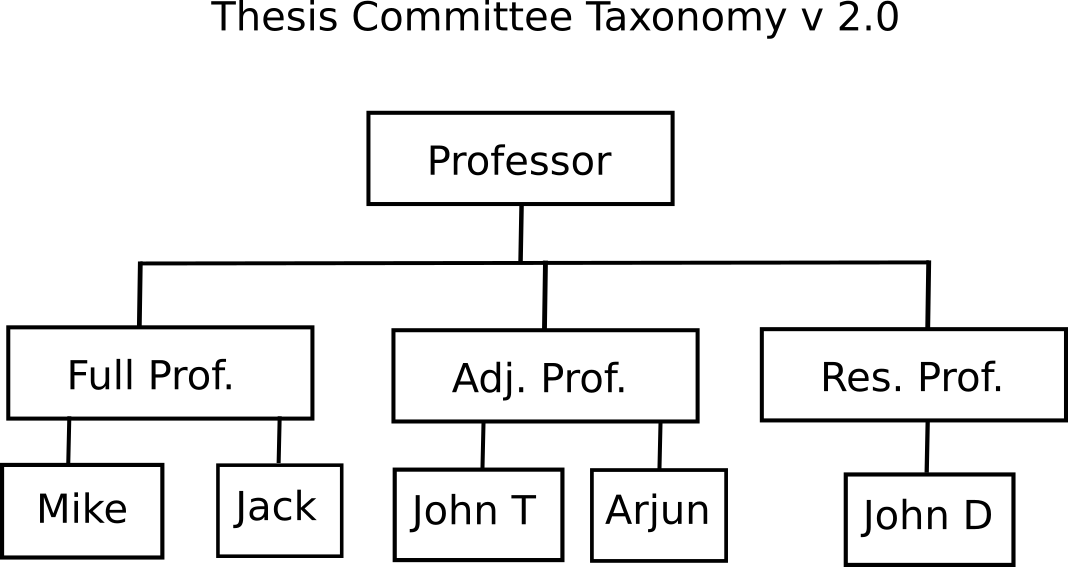
\includegraphics[width=\textwidth]{figures/tc-tax-v2.png}
\caption{Simple taxonomy of the professors and their ranks as described
in \S \ref{case-study}.}
\label{tax-1}
\end{figure}

Figure \ref{tax-2} includes the facts from all six statements. The red ``X''
marks in this figure indicate where the single relationship rule of a taxonomy
has been broken. First, in a taxonomy, all guitarists would inherit from the
same parent, or from multiple guitar-playing parents who inherit from another
guitar-playing grandparent. Second, although Mike Jr. is Mike's son
and a full professor, Mike Jr. is not a businessman and a pilot. Finally, the
relationship types between the professors, their bases classes, and the
additional occupational and familial classifications change throughout the
taxonomy in an unclear way.

\begin{figure}[htbp]
\centering
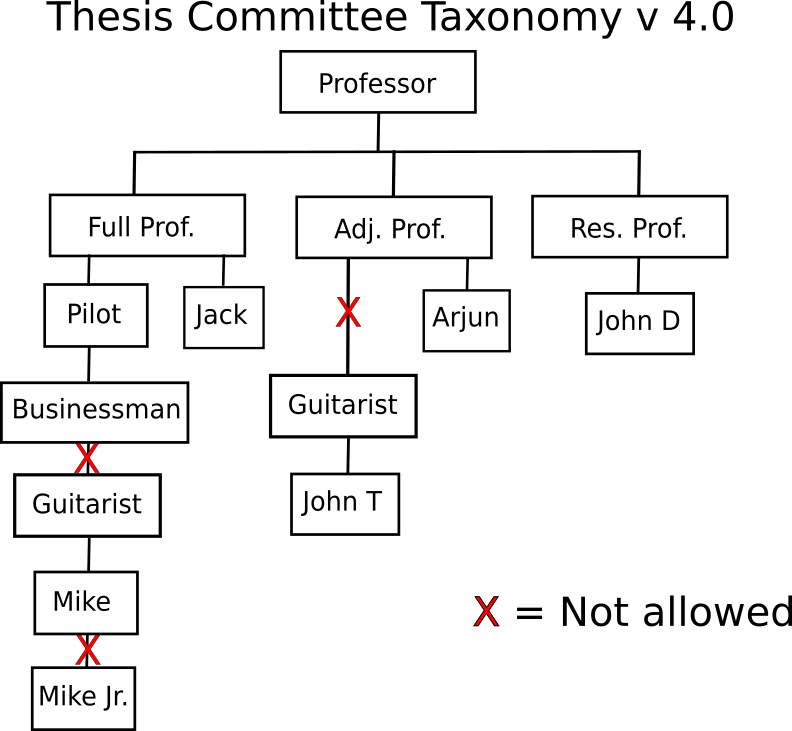
\includegraphics[width=\textwidth]{figures/tc-tax-v4-wErrors.png}
\caption{``Complete'' attempt at encoding the facts in \S \ref{case-study}.
The red ``X'' marks indicate the types of relationships that are not allowed
under the rules of a taxonomy.} 
\label{tax-2}
\end{figure}

These issues illustrate the fundamental problem with a taxonomy for
heterogeneous knowledge capture: ``Basic'' taxonomies only allow single direct
inheritance relationships to be expressed. This can be partially fixed by
allowing the relationship type to be changed based on an in-line annotation, but
what about properties such as ``can play guitar?'' Conceptually ``can play
guitar'' is not the same type of relationship as an ``is-a'' relationship. Is
a special annotation or graphic required for each new property type?
Furthermore, how does one rectify the fact that not all full professors are in
business, fly planes, or play guitar? What if a research professor did those
things as well? The complexity of the required modified taxonomy creates such a
complex diagram that one might as well simply leave the statements written
instead of encoded!

As more changes to the fundamental taxonomic data structure are required, the
required formality and bookkeeping also increase. It quickly becomes necessary
to create a separate structure simply for the purposes of managing all the
bookkeeping. Then, the data structure that uses the bookkeeping data structure
becomes something that uses the bookkeeping relationships to encode the facts.
A complex bookkeeping structure of this type that can encode classes,
relationships, and properties is an ontology, and the accompanying structure,
the graph of individuals, is known commonly as an \textit{instance graph},
\textit{knowledge graph}, or just graph of members or instances of the
ontology.

A simple ontology that describes the types of relationships, properties, and
classes for the six statements is shown in Figure \ref{ont-classes}.
Notice that this ontology contains a simple taxonomy of classes who are
Persons. Unlike the original taxonomy, Businessman, Guitarist, Pilot,
and Professor are all peers. The ontology has the following properties:
\begin{itemize}
  \item isFullProf - individuals with this property are Full Professors
  \item isAdjProf - individuals with this property are Adjunct Professors
  \item isResProf - individuals with this property are Research Professors
  \item hasSon - individuals with this property have a son whose identity is the
  object of the property
\end{itemize} 
The isFullProf, isAdjProf, and isResProf properties are all Boolean properties
that are either true or false. The \textit{hasSon} property is somewhat special
compared with the others because it encodes a relationship as a property. These
types of properties need to indicate clearly where they originate in the graph
and where they end. For statement 5 this could be indicated on the instance
graph by a property with a value of ``Mike Jr.'' or a graphic indication linking
Mike and Mike Jr.

The ontology also has the following \textit{disjoint} properties:
\begin{itemize}
  \item isFullProf != isAdjProf
  \item isFullProf != isResProf
  \item isAdjProf != isResProf
\end{itemize}
where the ``!='' indicates a negation relationship meaning ``is not.'' The
disjoint properties constrain the relationships between the normal properties
for semantic purposes. Subclasses are usually disjoint.

\begin{figure}[htbp]
\centering
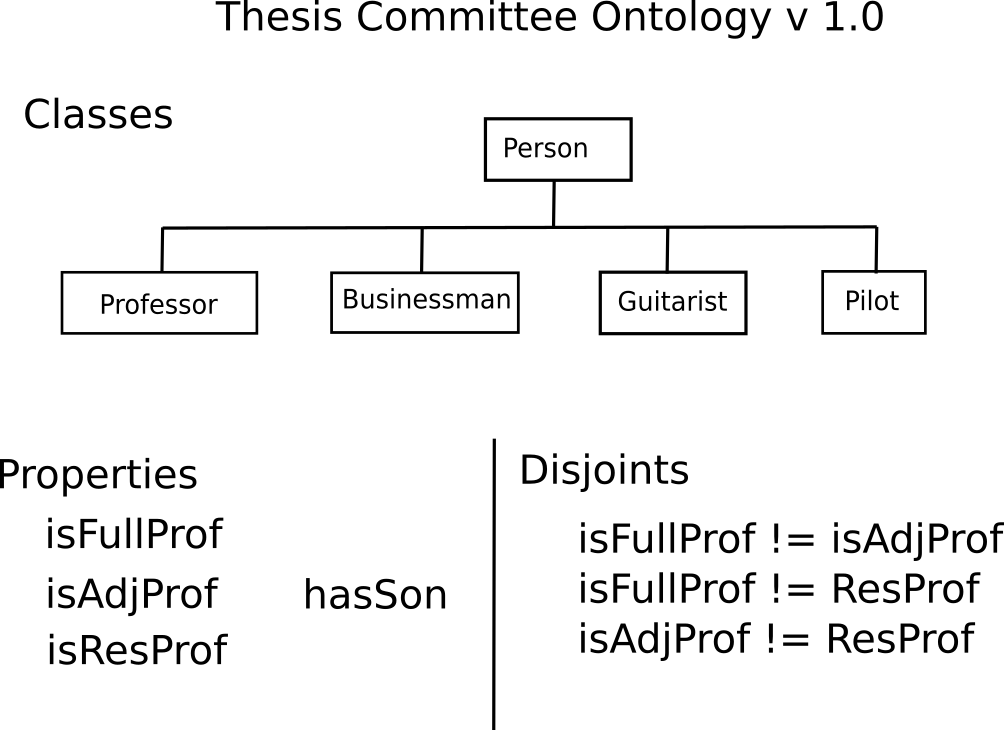
\includegraphics[width=\textwidth]{figures/tc-ont-classes.png}
\caption{Relationships, properties, and classes for the example in \S
\ref{case-study}.}
\label{ont-classes}
\end{figure}

The instance graph that uses the ontology to encode all six statements is shown
in Figure \ref{ont-instances}. This graph combines taxonomic ``is-a''
relationships and the ontological properties to fully represent the facts
and removes the representational problems found in Figure \ref{tax-2}. This
includes Mike's multiple roles and parental status. Professorial rank is
captured with properties instead of through direct inheritance. Note that the
green line in this figure has no special significance, but its color is useful
to show its path next to the black lines.

\begin{figure}[htbp]
\centering
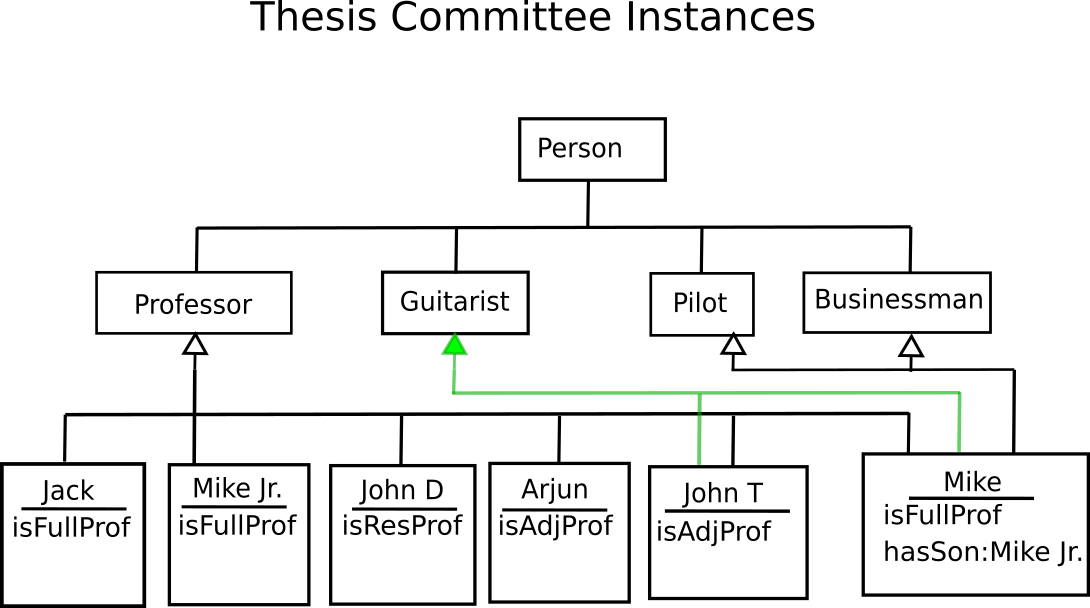
\includegraphics[width=\textwidth]{figures/tc-ont-instances.png}
\caption{Instance graph that uses the ontology in Figure \ref{ont-classes}
to encode the example in \S \ref{case-study}. The green line is not of
ontological signficnance but is colored separately to show the full connection.}
\label{ont-instances}
\end{figure}

An important aspect of ontologies, including this example, is that new facts
that are not present in the instance graph can often be inferred from the facts that
are present. Alternatively, because the graphs are open, merging graphs can
reveal new facts when inference rules are applied. Two facts that can be
inferred from the present set of facts is that an inverse relationship exists
for ``hasSon,'' which we might obviously call ``hasFather,'' and the identity of
Mike Jr.'s father is Mike. These facts are obvious to human readers, but that is
only because our experience fills in the ontological gaps. With respect to graph
mergers revealing new facts, suppose that someone merged a new ontology that
described Persons in great detail and that one property it described is that
all sons are male. It would then be possible to immediately deduce that Mike Jr.
is male.

\section{Machine Readable Ontologies}

Real life ontologies are significantly more complex than the example in \S
\ref{case-study}. They are also used to capture and reason about large sets of
facts, which requires computational resources for processing. It is not feasible
to create any such ontology using the scheme in the example, and numerous
ontological standards have been developed. 

OWL and related languages are used for this work to
capture ontological details in a machine readable way without sacrificing any
formality that is also useful to the human reader. OWL is based on RDFS, which
is in turn based on RDF.

Summaries of these languages are provided below based on the most recent
langauge specifications and other sources, \cite{allemang_semantic_2008}. These
summaries also include practical findings from the author who as a user of
these languages discovered a number of pitfalls that are not commonly or widely
discussed in the extant literature.

\subsection{The Resource Description Framework}

RDF is a W3C standard for exchanging data
across the internet \cite{noauthor_rdf_nodate}\cite{noauthor_rdf_nodate-3}. It
forms the basis of a so-called \textit{semantic web} where data resources are both linked and
self-describing, thus making large knowledge graphs that can be easily walked
to understand and find meaning in data.

The key concept in RDF is that statements can be made about uniquely
identifiable \textit{resources} in human and machine readable ways. Resources
are uniquely identified with internationalized resource identifiers (IRIs) that
extend the universal resource identifier (URI) standard by adding support for
non-English characters and non-ASCII character sets. Resource names can be
anything from simple names that are locally unique to fully qualified globally
unique names.

Descriptions of resources are made with statements. Statements in RDF are
similar to sentences in the English language. Each statement contains a subject,
predicate, and object. The predicate describes the relationship of the subject
to the object in an RDF statement, just as the predicate (verb) ``is'' links the
subject ``color'' (or ``ballColor'') to the object ``red'' in ``The color of
the ball is red.'' This type of statement is called a \textit{triple}.

RDF triples are represented as full graph data structures in memory and are
serialized to any one of a number of file formats, including an XML-based format
and several formats that are easier for humans to read \cite{noauthor_resource_2019}.
Most of the supported formats for RDF are standardized, although several formats
add support for additional features not found in the standard. This includes the
JSON Linked Data (JSON-LD) and Notation3 formats. Unless otherwise
specified, the remainder of this document uses a very readable and common
serialization called the Terse RDF Triple Language (TURTL)
\cite{noauthor_rdf_nodate-4}. This format is signifcantly easier to understand
than others for humans and has the added advantage of being succinct in written
text. For example, the statement ``The color of the ball is red'' would be
rendered as a TURTLE triple with \begin{lstlisting}[language=TURTL]
<#ball>
    hasColor <red>.
\end{lstlisting}
whereas for an RDF/XML triple it would be
\begin{lstlisting}[language=XML]
<?xml version="1.0"?>
<RDF>
  <Description about="ball">
    <hasColor>red</hasColor>
  </Description>
</RDF>
\end{lstlisting}

Statements about resources can be distributed, including outside of their
current graph. In the RDF literature, this is described by the phrase ``Anyone
can say anything about anything'' (AAA). This means that for any given resource,
any other resource can be included in triples. This is akin to the ontological
openness described in \S \ref{ont-openess}. This also means that without human
intervention it is very hard to establish the origin of data for which there are
numerous distributed triples, unless one of those triples provides such a
description. Within the current graph, resource descriptions can be segmented
for clarity. If a statement such as ``Jay Jay Billings works at Oak Ridge
National Laboratory, a DOE facility,'' is made, instead of writing a single
TURTL triple that captures all the facts, it could be written as
\begin{lstlisting}[language=TURTL] <#JayJayBillings>
    worksAt <#ORNL>.
<#ORNL>
    a <#NationalLaboratory>; hasName ``Oak Ridge National
    Laboratory''^^xsd:string.,
\end{lstlisting}
which uses references to other triples and links them into the original triple
about the author.

Notice the previous listing includes the term
\begin{lstlisting}[language=TURTL]
    hasName ``Oak Ridge National Laboratory''^^xsd:string.
\end{lstlisting}
This term assigns a \textit{literal} value of ``Oak Ridge National Laboratory''
to the subject of the triple. The additional characters at the end ---
``\textasciicircum\textasciicircum xsd:string''--- set the type of the literal
to an XML schema definition string. Literal values can be set for many different types of data, including
most primitives such as integers and floating point numbers found in standard
programming languages.

Section \ref{case-study} briefly mentions the process of inference. Basic RDF
is straightforward: it describes resources. However, it is possible to include data
on the resources that establishes the relationships among them and thus makes
it possible to infer facts that are not explicitly written
\cite{allemang_semantic_2008}. This can include data shaping to conform to a
particular set of information, type restriction, or classification information.
These capabilities are provided as languages built on top of RDF, including the
RDFS and OWL.

An important aspect of RDF not covered in more detail in this work is the
ability to query it using the SPARQL query language. 

\todo{GET NOTES FROM NOTEBOOK!!!!\\}

\subsubsection{Containers}

RDF has several \textit{containers} that can hold sets of data
\cite{noauthor_rdf_nodate-3}. These include rdfs:Container, rdf:Bag, rdf:Seq,
and rdf:Alt. These containers are considered to be open, and additional data can
be added. Alternative closed containers called \textit{collections} represent
sets of data that cannot be modified and that are ordered from first to last
element. The only supported collection in the RDF specification is rdf:List.

Containers and collections are signficantly different than similarly named
structures in object-oriented programming languages, especially where generic
and templated programming is concerned.

\subsection{RDFS}

Although programming languages have preset grammars, data languages are often
left without a language that describes in machine readable terms the allowed
values and entries in a data file. This information is provided for users in
a format specification for the data language but not in a way that can be
programmatically enforced. 

RDFS provides this capability for RDF \cite{noauthor_rdf_nodate-5}\cite{
allemang_semantic_2008}. RDFS supports describing sets of RDF resources in a
machine readable way that can subsequently be used for validation and inference.
RDFS is itself defined in RDF, so the sets, or classes, of resources defined by
the schema are described in a standard RDF file, as are instance files
containing data that conforms to the schema.

Classes in RDFS are described by the rdfs:class descriptor in a triple. For
example,
\begin{lstlisting}[language=TURTL]
<#cat>
    rdf:type rdfs:Class;
\end{lstlisting}
defines a type of class called Cat. The rdf:type predicate is a special
statement that indicates the type of resource is specified by the
object. 

RDFS classes also support inheritance, and ``Cat'' could inherit from
``Mammal'' or ``Feline,'' as expected. The following TURTL triple illustrates
that:
\begin{lstlisting}[language=TURTL]
<#cat>
    rdfs:subClassOf <Mammal>.
\end{lstlisting}
It is also possible for properties to inherit from other properties using the
rdfs:subPropertyOf relation.

Likewise, individuals can be declared to be of a particular type. The TURTL
triple
\begin{lstlisting}[language=TURTL]
<#garfield>
    rdf:type <#cat>;
    hasName  ``Garfield''^^xsd:string.
\end{lstlisting}
describes a cat named Garfield, which we can infer to be a mammal as well.

The rdfs:subClassOf term used for inheritance is actually a property. To put
this differently, the subject of a triple with the predicate rdfs:subClassOf
has the property that it is a subclass of the other class. 

Triples are in general just maps of subjects and objects via properties.
Sometimes it is necessary to restrict what type of subject relates to a
particular type of object in this mapping. In this case, the rdfs:domain and
rdfs:range properties can be used to restrict the types of the root property.
The rdfs:domain property restricts the type of a subject, while the rdfs:range
property restricts the type of an object. It is possible to simultaneously
define rdfs:domain and rdfs:range for a property.

A select number of logic operations are supported by RDFS, including unions and
intersections. Special relations exist for the logic operations for classes and
properties alike.

Many schemas exist for reuse on the internet and are available for
public download through sites like Linked Data Applications
\cite{noauthor_linked_nodate-1}. These schemas can be included through an
approriate import call in the RDF file. In TURTL, imports are handled with the ``@prefix''
statement, as follows:
\begin{lstlisting}[language=TURTL]
@prefix rdfs: <http://www.w3.org/2000/01/rdf-schema#> .
@prefix foaf: <http://xmlns.com/foaf/0.1/> .

<#banana>
    rdf:type rdfs:Class;
    foaf:knows ``Spongebob''.,
\end{lstlisting}
where \textit{rdfs} and \textit{foaf} are imported schemas.

One nice feature of RDFS that is completely nonfunctional but useful
nonetheless is the addition of rdfs:Comment and rdfs:Label relations that make
it possible to provide detailed comments describing the data, as well as a
user-friendly label that can be substituted for default or missing data by the
display.

RDFS adds powerful features to the RDF language stack. However, as powerful as
it is, many different types of relations are missing, which restricts its
utility for more complex data relationships. Luckily, these and more are
available in OWL.

\subsection{Web Ontology Language}

OWL builds on RDF and RDFS to add additional
features for inferencing and formal ontological syntax \cite{
noauthor_owl_nodate}. The major addition to OWL over RDFS is a set of
properties that describe inverse, transitive, symmetric, and equivalent relationships
\cite{allemang_semantic_2008}. Unlike RDF and RDFS, the primary purpose of OWL
it to provide enough semantic constructs so that inferencing can be greatly
expanded for well-described data. This makes it possible for instance data that
follows an OWL ontology to be very well understood based solely on the provided
data set and the ontology.

OWL's set of default properties can be extended very easily to create new
ontological constructs by mixing the default properties in new ways. Since OWL
is serialized using RDF (which is not a strict requirement) extension is
performed simply by creating a new RDF triple that links the relevant terms.

Modeling ontologies with OWL is different than modeling in languages such as the
UML. There are many subtle differences
between the two languages, but UML is more general. In fact, OWL is
defined in part with UML models. One additional difference of particular
importance is that classes in UML can have member variables that are tied
directly to a single class. It is possible to emulate this behavior in OWL
through object properties and the rdfs:domain and rdfs:range properties that
restrict the type subject and predicate types, but without these restrictions
object properties can be used by any class. Additionally, complex members
may require pointer-like object properties linking them to their class. OWL also
allows properties to have properties, including transitive properties, which is
generally reserved only for classes in object-oriented languages.

There are several different types of OWL that can be selected based on the
preferred inference needs of the client. Since general graphs can be
computationally costly to search thoroughly, ``lighter'' versions of the
specifications with properties removed can be much faster if the data will allow
it. The complete version of OWL is commonly called OWL Full or just OWL. The two
sublanguages of OWL are OWL Lite and OWL DL. OWL Lite is a lightweight subset
of OWL on which inferencing models can be run very quickly. OWL DL
is a middle ground in terms of feature richness and performance
during inferencing \cite{noauthor_owl_nodate-2}.

\subsection{Useful Tools}

There are numerous tools, many of which are exceptional, for working with linked
data and semantic web technologies. This section provides a summary of some of
these tools, not as an endorsement but as a reference for the interested reader.

\subsubsection{Linked Open Vocabularies}

The Linked Open Vocabularies (LOV) project is a repository for ontologies from
the Ontology Engineering Group \cite{noauthor_linked_nodate-1}. The site
provides up-to-date information on ontologies and vocabularies for a large number of projects, all
of which is searchable and can be examined with a friendly web interface. This
repository can be used to find high-quality, well-tested resources instead of
writing new ones from scratch.

\subsubsection{Prot\'eg\'e}

Prot\'eg\'e is an open source ontology editor created by the Stanford Center for
Biomedical Informatics Research at the Stanford University School of Medicine
\cite{noauthor_protege_nodate}. Ontologies can be managed as individual files or
as part of version control repositories. In addition to providing general creation and
editorial support for ontologies, Prot\'eg\'e includes a large number of plugins
that provide extra tools such as visualization engines and documentation
exporters.

All of the ontologies in this work were created using Prot\'eg\'e, with only
minor edits and some initial learning work performed in different tools. This
includes the original versions of graphs shown later in the text.

\subsubsection{Apache Jena}

Apache Jena is an open source framework that supports six different projects for
semantic web and linked data applications \cite{noauthor_apache_nodate-1}. These
include an RDF utility library and SPARQL query engine, a file-based and a web-based
triple store, and ontology and inference libraries. Apache Jena is written in
Java, although the web-based triple store is available by standard HTTP calls. 
Apache Jena is very useful for writing programs that can directly manipulate
RDF resources, including storing the graphs for later use.

\subsubsection{Eclipse}

The Eclipse Platform is an open source platform that has more than 300
projects, managed by the Eclipse Foundation. The
platform includes many different tools, including a generic XML editor
that is very good for RDF/XML files and a TURTL editor, that is available as a
third-party plugin \cite{ noauthor_xturtle_nodate}. The platform includes
additional tools for managing basic file manipulation for ontologies and RDF
data. It also includes tools for managing software and data repositories. The
majority of this dissertation was written using the Texlipse plugin to Eclipse.

\subsubsection{Graphviz}

Graphviz is a powerful graph visualization tool that supports the Dot language
\cite{noauthor_graphviz_nodate}. Nodes in graphs are drawn as circles with
labels and connections between the nodes are drawn as curves with annotations
that describe their connection type. This is very useful for RDF graphs where
both the node types and connections vary depending on the details of the triple.

\subsection{Our Case Study in RDF and OWL}

\begin{figure}[htbp]
\centering
\baseIncludegraphics{exampleOntology/exampleOntology.png}
\caption{Graphviz plot of the combined thesis committee ontology and its
individuals.}
\label{example-ont-graphic}
\end{figure}

The previous sections provide all that is needed to create a simple,
formal, machine readable ontology for the thesis committee example at the
beginning of this chapter. As a pedagogical tool, that example is fine, but as
an example of a real ontology it suffers from being written by just another guy
in his arm chair! Using the tools of the previous section, it can be turned
into something very similar to what will be developed for scientific workflows,
as well as ontologies commonly available in the LOV
repository. Figure \ref{example-ont-graphic} shows the committee ontology and
its individuals rendered in a single Graphviz graph. Listing
\ref{example-ont-listing} shows the same content as the graph but in its
formal TURTL serialization.

\lstinputlisting[language=TURTL,caption=The complete OWL ontology
for the example problem.,label=example-ont-listing]{/home/bkj/thesis/exampleOntology/exampleOntology.turtl.owl}

The ontology and its individuals were created completely in Prot\'eg\'e using an
in-memory representation of the graph. Exports were created for both the
Graphviz plot and the TURTL file. Apache Jena can readily consume the TURTL file
for further processing.

\section{Summary}

This chapter introduces the concept of an ontology, including its common
features and the fundamental differences between ontologies and taxonomies. A
simple example is presented that shows how even simple relationships can be
difficult to capture without the formalism and reasoning abilities of
ontological tools.

The RDF-based languages for working with RDF, RDFS, and OWL are described with
a particular focus on those features that are most useful to this work. Useful
tools for creating ontologies and RDF models are also presented.

Finally, the original committee example was revisited using the tools and
techniques described for the RDF-based languages. This introduces formality,
structure, and machine-readable properties that put the example, as simple as it
is, on par with ontologies of much broader appeal.

Using the languages and tools presented in this chapter, and the description of
scientific workflows and workflow engines provided elsewhere in this work, it is
now possible to pursue the goal of creating an ontology that accurately
describes the phantasmagoria of scientific workflows.
